\documentclass[11pt]{article}            % Report class in 11 points
\parindent0pt  \parskip10pt             % make block paragraphs
\usepackage{graphicx}
\usepackage{listings}
\graphicspath{ {images/} }
\usepackage{graphicx} %  graphics header file
\begin{document}
\begin{titlepage}
    \centering
  \vfill
    
\includegraphics[width=8cm]{uni_logo.png} \\ 
	\vskip2cm
    {\bfseries\Large
	Data Structures and algorythm  \\ (CS09203)\\
	
	\vskip2cm
	Lab Report 
	 
	\vskip2cm
	}    

\begin{center}
\begin{tabular}{ l l  } 

Name: & MuhammadTalhaKhalid \\ 
Registration \#: &CSU-S16-135\\ 
Lab Report \#: & 1 \\ 
 Dated:& 13-04-2018\\ 
Submitted To:& Mr. Usman Ahmed\\ 

 %\hline
\end{tabular}
\end{center}
    \vfill
    The University of Lahore, Islamabad Campus\\
Department of Computer Science \& Information Technology
\end{titlepage}


    
    {\bfseries\Large
\centering
	Experiment \# 1 \\

Data Handeling into an array\\
	
	}    
 \vskip1cm
 \textbf {Objective}\\  To understand How to Handle data into array .
 
 \textbf {Software Tool} \\
1. Microsof Windows 7 \\
2. Dev c++\\
3. Miktext editor \\

\section{Theory }              
In this experiment we learn how to handle our data using and array and basic concept of link listing using arrays \\
It has 3 rules:\\
1.	Input our data into array.\\
2.	Replace our data to certain place on array .\\ 
3.	move the element of the location which we replace and move it to next spot on array.\\ \\ 

\section{Task}  
\subsection{Procedure: Task 1 }     

\begin{figure*}
\centering
  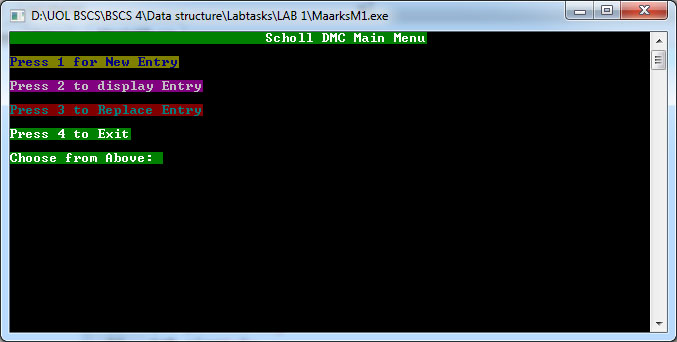
\includegraphics[width=12cm,height=6cm,keepaspectratio]{1.jpg}
\caption{Main menu of my program}
\label{Figure:1}    
  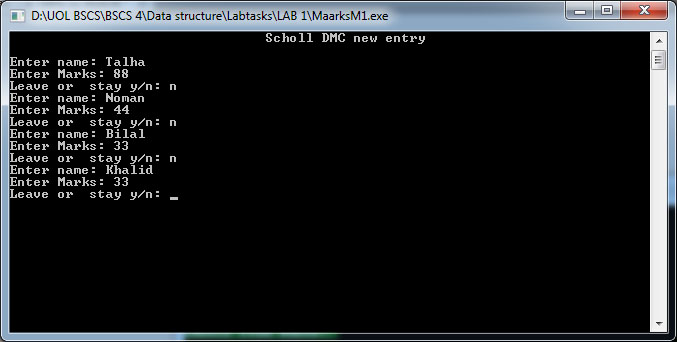
\includegraphics[width=12cm,height=6cm,keepaspectratio]{2.jpg}
\caption{New entry into array}
\label{Figure:2}   
\end{figure*}
In this We eter our data into nd  arry which is students names and there marks



\subsection{Procedure: Task 2 }     
\begin{lstlisting}[language=C++]

#include<stdio.h>
#include<iostream>
#include<dos.h>
#include<unistd.h>
#include<string>
#include<stdlib.h>
#include<Loadanim.h>
using namespace std;
string names[100];
int marks[100];
//Edit marks datatype
string EditName="\0";
int  EditMarks;
//Position and size
int position=0;
int size=-1;
string Exit;

void InputMarks() { //New marks entry
	do {
		size++;
		cout<<"Enter name: ";
		cin>>names[size];
		cout<<"Enter Marks: ";
		cin>>marks[size];
		
		cout<<"Leave or  stay y/n: ";
		cin>>Exit;
	}while(Exit!="y");
}//End of input markd

void Display() {//Dsiplay Current Marrks
	do {
	for(int i=0;i<size+1;i++) {
		cout<<i<<":) "<<names[i]<<"\t\t"<<marks[i]<<endl;
	}
	cout<<"Wana exit y/n: ";
	cin>>Exit;
      }while(Exit!="y");
	
}//End of Display

void Replace() { //replace Marks
system("cls");
do {
		do {
			system("cls");
	Display();
	cout<<"Choosse number from above u wana Replace: ";
	cin>>position;
	if(position>=size) {
		cerr<<"error!! not found\n";
		system("pause");
			}
		}while(position>=size);
	cout<<"Enter new name";
	cin>>EditName;
	cout<<"Enter new Marks";
	cin>>EditMarks;
	/*for(int i=size;i>position;i--) {
		names[i]=names[i-1];
		names[size]=EditName;
		marks[i]=marks[i-1];
		marks[size]=EditMarks;
	}*/
	names[position]=EditName;
	marks[position]=EditMarks;
	cout<<"WANT TO EXIT y/n";
	cin>>Exit;
		}while(Exit!="y");
	
}//end of marks replacement

void list() {
	ColorInput Ci;
	system("cls");
	Ci.CustColor("\t\t\t\tScholl DMC Main Menu\n\n",47);
	Ci.CustColor("Press 1 for New Entry\n\n",97);
	Ci.CustColor("Press 2 to display Entry\n\n",87);
	Ci.CustColor("Press 3 to Replace Entry\n\n",67);
	Ci.CustColor("Press 4 to Exit\n\n",47);
}

int main()//Main 
{
	LoadAnimate la;
	la.Loading(4,33);
	int choice;
	ColorInput Ci;
	system("cls");
	do {
	list();
		Ci.CustColor("Choose from Above: ",47);
	cin>>choice;
 cout<<Ci;
	switch (choice) {
		case 1://New entry
		la.Loading(2,47);
		system("cls");
		cout<<"\t\t\t\tScholl DMC new entry\n\n";
			InputMarks();
			break;
			
			case 2://Display
			la.Loading(2,27);
			system("cls");
				cout<<"\t\t\t\tScholl Marks Sheet\n\n";
				cout<<"Names\t\t\tMarks\n";
				Display();
				
				break;
				
				case 3://replacement
				la.Loading(2,27);
					system("cls");
					cout<<"\t\t\t\tReplace Marks\n\n";
					Replace();
					break;
	}
	}while(choice!=4);
	return 0;   }
\end{lstlisting}
\begin{figure*}
\section{Output: }
\centering
  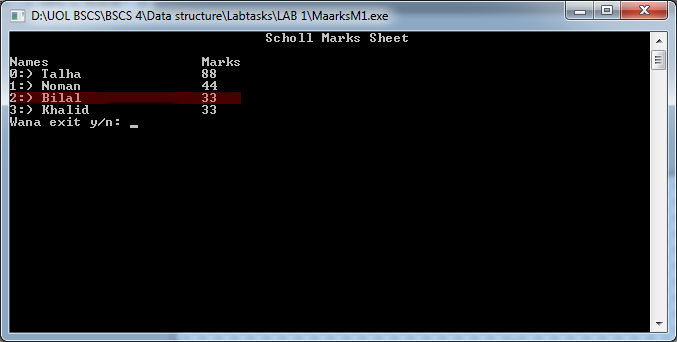
\includegraphics[width=12cm,height=6cm,keepaspectratio]{3.jpg}
\caption{Display output of my Stored Data}
\label{Figure:3}   
 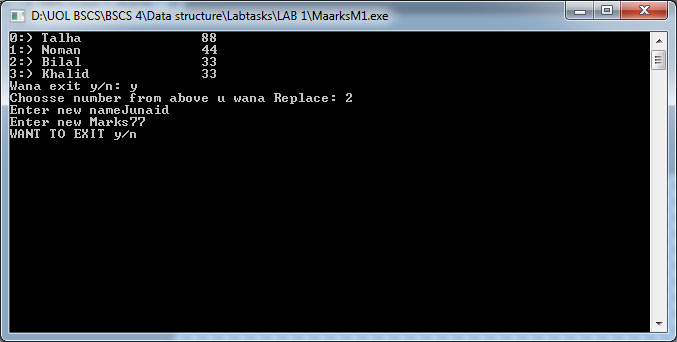
\includegraphics[width=12cm,height=6cm,keepaspectratio]{5.jpg}
\caption{Replace no array loacation Bilal With Junaid}
\label{Figure:4}
\end{figure*}
\begin{figure*}
 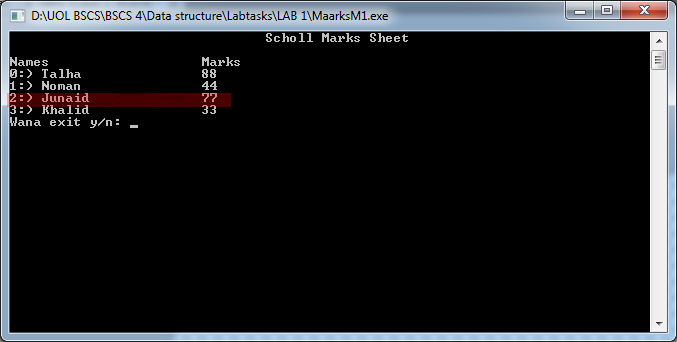
\includegraphics[width=12cm,height=6cm,keepaspectratio]{6.jpg}
\caption{Replaced Bilal with junaid in arrray location 2}
\label{Figure:5}
\section{Conclusion:}  
so we learn from this program that how to enter our data into an array,how to shift the data on specific Location to next array and put new data and this program also leads us to concept of link listing  \\
We can implement  it with object oriented programming where we can add a new object of certain class  and work on it and replace a whole object of that with other class\\
\end{figure*}

\end{document}                          % The required last line
